% Created by tikzDevice version 0.12.6 on 2025-03-13 14:19:40
% !TEX encoding = UTF-8 Unicode
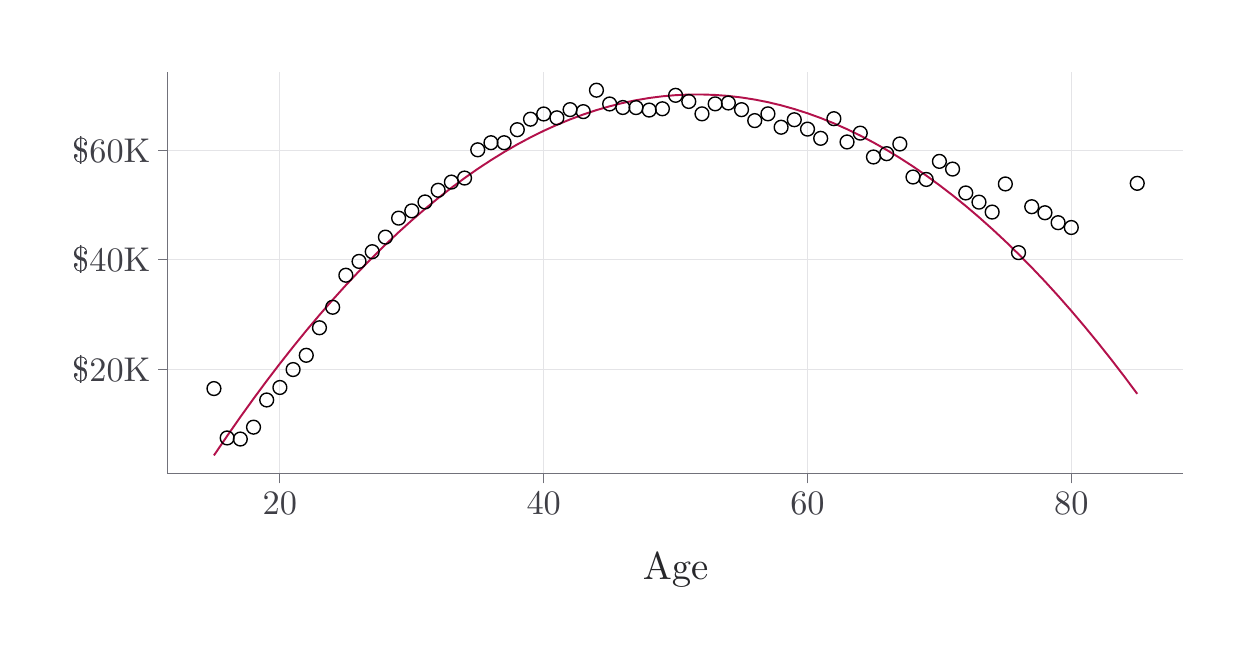
\begin{tikzpicture}[x=1pt,y=1pt]
\definecolor{fillColor}{RGB}{255,255,255}
\path[use as bounding box,fill=fillColor] (0,0) rectangle (433.62,216.81);
\begin{scope}
\path[clip] (  0.00,  0.00) rectangle (433.62,216.81);
\definecolor{drawColor}{RGB}{255,255,255}

\path[draw=drawColor,line width= 0.7pt,line join=round,line cap=round,fill=fillColor] ( -0.00,  0.00) rectangle (433.62,216.81);
\end{scope}
\begin{scope}
\path[clip] ( 50.63, 55.65) rectangle (417.62,200.81);
\definecolor{drawColor}{RGB}{255,255,255}
\definecolor{fillColor}{RGB}{255,255,255}

\path[draw=drawColor,line width= 0.7pt,line join=round,line cap=round,fill=fillColor] ( 50.63, 55.65) rectangle (417.62,200.81);
\definecolor{drawColor}{RGB}{228,228,231}

\path[draw=drawColor,line width= 0.4pt,line join=round] ( 50.63, 93.39) --
	(417.62, 93.39);

\path[draw=drawColor,line width= 0.4pt,line join=round] ( 50.63,132.90) --
	(417.62,132.90);

\path[draw=drawColor,line width= 0.4pt,line join=round] ( 50.63,172.40) --
	(417.62,172.40);

\path[draw=drawColor,line width= 0.4pt,line join=round] ( 91.14, 55.65) --
	( 91.14,200.81);

\path[draw=drawColor,line width= 0.4pt,line join=round] (186.46, 55.65) --
	(186.46,200.81);

\path[draw=drawColor,line width= 0.4pt,line join=round] (281.79, 55.65) --
	(281.79,200.81);

\path[draw=drawColor,line width= 0.4pt,line join=round] (377.11, 55.65) --
	(377.11,200.81);
\definecolor{drawColor}{RGB}{179,17,75}

\path[draw=drawColor,line width= 0.7pt,line join=round] ( 67.31, 62.25) --
	( 72.08, 69.27) --
	( 76.84, 76.10) --
	( 81.61, 82.74) --
	( 86.37, 89.18) --
	( 91.14, 95.42) --
	( 95.91,101.47) --
	(100.67,107.33) --
	(105.44,112.99) --
	(110.21,118.46) --
	(114.97,123.74) --
	(119.74,128.82) --
	(124.50,133.70) --
	(129.27,138.39) --
	(134.04,142.89) --
	(138.80,147.19) --
	(143.57,151.30) --
	(148.33,155.22) --
	(153.10,158.93) --
	(157.87,162.46) --
	(162.63,165.79) --
	(167.40,168.93) --
	(172.16,171.87) --
	(176.93,174.62) --
	(181.70,177.17) --
	(186.46,179.53) --
	(191.23,181.69) --
	(196.00,183.66) --
	(200.76,185.44) --
	(205.53,187.02) --
	(210.29,188.40) --
	(215.06,189.60) --
	(219.83,190.60) --
	(224.59,191.40) --
	(229.36,192.01) --
	(234.12,192.42) --
	(238.89,192.64) --
	(243.66,192.67) --
	(248.42,192.50) --
	(253.19,192.14) --
	(257.95,191.58) --
	(262.72,190.83) --
	(267.49,189.89) --
	(272.25,188.75) --
	(277.02,187.41) --
	(281.79,185.88) --
	(286.55,184.16) --
	(291.32,182.24) --
	(296.08,180.13) --
	(300.85,177.82) --
	(305.62,175.32) --
	(310.38,172.63) --
	(315.15,169.74) --
	(319.91,166.66) --
	(324.68,163.38) --
	(329.45,159.90) --
	(334.21,156.24) --
	(338.98,152.38) --
	(343.75,148.32) --
	(348.51,144.07) --
	(353.28,139.63) --
	(358.04,134.99) --
	(362.81,130.15) --
	(367.58,125.13) --
	(372.34,119.91) --
	(377.11,114.49) --
	(381.87,108.88) --
	(386.64,103.07) --
	(391.41, 97.07) --
	(396.17, 90.88) --
	(400.94, 84.49);
\definecolor{drawColor}{RGB}{0,0,0}

\path[draw=drawColor,line width= 0.5pt,line join=round,line cap=round] (257.95,187.18) circle (  2.50);

\path[draw=drawColor,line width= 0.5pt,line join=round,line cap=round] (196.00,187.20) circle (  2.50);

\path[draw=drawColor,line width= 0.5pt,line join=round,line cap=round] ( 95.91, 93.27) circle (  2.50);

\path[draw=drawColor,line width= 0.5pt,line join=round,line cap=round] (277.02,183.54) circle (  2.50);

\path[draw=drawColor,line width= 0.5pt,line join=round,line cap=round] (281.79,180.15) circle (  2.50);

\path[draw=drawColor,line width= 0.5pt,line join=round,line cap=round] (129.27,141.12) circle (  2.50);

\path[draw=drawColor,line width= 0.5pt,line join=round,line cap=round] (134.04,147.98) circle (  2.50);

\path[draw=drawColor,line width= 0.5pt,line join=round,line cap=round] (291.32,183.92) circle (  2.50);

\path[draw=drawColor,line width= 0.5pt,line join=round,line cap=round] (238.89,190.14) circle (  2.50);

\path[draw=drawColor,line width= 0.5pt,line join=round,line cap=round] (210.29,189.23) circle (  2.50);

\path[draw=drawColor,line width= 0.5pt,line join=round,line cap=round] ( 76.84, 68.16) circle (  2.50);

\path[draw=drawColor,line width= 0.5pt,line join=round,line cap=round] (272.25,180.83) circle (  2.50);

\path[draw=drawColor,line width= 0.5pt,line join=round,line cap=round] (253.19,189.59) circle (  2.50);

\path[draw=drawColor,line width= 0.5pt,line join=round,line cap=round] (305.62,170.08) circle (  2.50);

\path[draw=drawColor,line width= 0.5pt,line join=round,line cap=round] (181.70,183.74) circle (  2.50);

\path[draw=drawColor,line width= 0.5pt,line join=round,line cap=round] (172.16,175.23) circle (  2.50);

\path[draw=drawColor,line width= 0.5pt,line join=round,line cap=round] (296.08,175.51) circle (  2.50);

\path[draw=drawColor,line width= 0.5pt,line join=round,line cap=round] (234.12,192.36) circle (  2.50);

\path[draw=drawColor,line width= 0.5pt,line join=round,line cap=round] (124.50,135.86) circle (  2.50);

\path[draw=drawColor,line width= 0.5pt,line join=round,line cap=round] (200.76,186.47) circle (  2.50);

\path[draw=drawColor,line width= 0.5pt,line join=round,line cap=round] ( 86.37, 82.28) circle (  2.50);

\path[draw=drawColor,line width= 0.5pt,line join=round,line cap=round] (262.72,183.23) circle (  2.50);

\path[draw=drawColor,line width= 0.5pt,line join=round,line cap=round] (119.74,132.35) circle (  2.50);

\path[draw=drawColor,line width= 0.5pt,line join=round,line cap=round] (248.42,189.28) circle (  2.50);

\path[draw=drawColor,line width= 0.5pt,line join=round,line cap=round] (157.87,162.47) circle (  2.50);

\path[draw=drawColor,line width= 0.5pt,line join=round,line cap=round] (143.57,153.83) circle (  2.50);

\path[draw=drawColor,line width= 0.5pt,line join=round,line cap=round] (267.49,185.67) circle (  2.50);

\path[draw=drawColor,line width= 0.5pt,line join=round,line cap=round] (215.06,187.96) circle (  2.50);

\path[draw=drawColor,line width= 0.5pt,line join=round,line cap=round] (205.53,194.21) circle (  2.50);

\path[draw=drawColor,line width= 0.5pt,line join=round,line cap=round] (310.38,171.28) circle (  2.50);

\path[draw=drawColor,line width= 0.5pt,line join=round,line cap=round] (138.80,150.61) circle (  2.50);

\path[draw=drawColor,line width= 0.5pt,line join=round,line cap=round] (148.33,158.05) circle (  2.50);

\path[draw=drawColor,line width= 0.5pt,line join=round,line cap=round] (167.40,175.24) circle (  2.50);

\path[draw=drawColor,line width= 0.5pt,line join=round,line cap=round] (324.68,161.96) circle (  2.50);

\path[draw=drawColor,line width= 0.5pt,line join=round,line cap=round] (153.10,161.01) circle (  2.50);

\path[draw=drawColor,line width= 0.5pt,line join=round,line cap=round] (229.36,187.50) circle (  2.50);

\path[draw=drawColor,line width= 0.5pt,line join=round,line cap=round] (100.67, 98.42) circle (  2.50);

\path[draw=drawColor,line width= 0.5pt,line join=round,line cap=round] (224.59,187.03) circle (  2.50);

\path[draw=drawColor,line width= 0.5pt,line join=round,line cap=round] (286.55,176.82) circle (  2.50);

\path[draw=drawColor,line width= 0.5pt,line join=round,line cap=round] (243.66,185.67) circle (  2.50);

\path[draw=drawColor,line width= 0.5pt,line join=round,line cap=round] (191.23,184.24) circle (  2.50);

\path[draw=drawColor,line width= 0.5pt,line join=round,line cap=round] (176.93,179.94) circle (  2.50);

\path[draw=drawColor,line width= 0.5pt,line join=round,line cap=round] ( 91.14, 86.79) circle (  2.50);

\path[draw=drawColor,line width= 0.5pt,line join=round,line cap=round] (219.83,187.92) circle (  2.50);

\path[draw=drawColor,line width= 0.5pt,line join=round,line cap=round] (162.63,172.67) circle (  2.50);

\path[draw=drawColor,line width= 0.5pt,line join=round,line cap=round] (110.21,115.78) circle (  2.50);

\path[draw=drawColor,line width= 0.5pt,line join=round,line cap=round] (300.85,178.70) circle (  2.50);

\path[draw=drawColor,line width= 0.5pt,line join=round,line cap=round] (105.44,108.37) circle (  2.50);

\path[draw=drawColor,line width= 0.5pt,line join=round,line cap=round] (343.75,153.76) circle (  2.50);

\path[draw=drawColor,line width= 0.5pt,line join=round,line cap=round] (362.81,152.11) circle (  2.50);

\path[draw=drawColor,line width= 0.5pt,line join=round,line cap=round] ( 72.08, 68.56) circle (  2.50);

\path[draw=drawColor,line width= 0.5pt,line join=round,line cap=round] (358.04,135.52) circle (  2.50);

\path[draw=drawColor,line width= 0.5pt,line join=round,line cap=round] (319.91,162.84) circle (  2.50);

\path[draw=drawColor,line width= 0.5pt,line join=round,line cap=round] ( 81.61, 72.45) circle (  2.50);

\path[draw=drawColor,line width= 0.5pt,line join=round,line cap=round] (186.46,185.62) circle (  2.50);

\path[draw=drawColor,line width= 0.5pt,line join=round,line cap=round] (114.97,127.35) circle (  2.50);

\path[draw=drawColor,line width= 0.5pt,line join=round,line cap=round] (353.28,160.34) circle (  2.50);

\path[draw=drawColor,line width= 0.5pt,line join=round,line cap=round] (338.98,157.08) circle (  2.50);

\path[draw=drawColor,line width= 0.5pt,line join=round,line cap=round] (315.15,174.78) circle (  2.50);

\path[draw=drawColor,line width= 0.5pt,line join=round,line cap=round] (334.21,165.71) circle (  2.50);

\path[draw=drawColor,line width= 0.5pt,line join=round,line cap=round] (348.51,150.17) circle (  2.50);

\path[draw=drawColor,line width= 0.5pt,line join=round,line cap=round] (329.45,168.49) circle (  2.50);

\path[draw=drawColor,line width= 0.5pt,line join=round,line cap=round] (377.11,144.60) circle (  2.50);

\path[draw=drawColor,line width= 0.5pt,line join=round,line cap=round] ( 67.31, 86.40) circle (  2.50);

\path[draw=drawColor,line width= 0.5pt,line join=round,line cap=round] (367.58,149.93) circle (  2.50);

\path[draw=drawColor,line width= 0.5pt,line join=round,line cap=round] (400.94,160.56) circle (  2.50);

\path[draw=drawColor,line width= 0.5pt,line join=round,line cap=round] (372.34,146.34) circle (  2.50);
\end{scope}
\begin{scope}
\path[clip] (  0.00,  0.00) rectangle (433.62,216.81);
\definecolor{drawColor}{RGB}{113,113,122}

\path[draw=drawColor,line width= 0.3pt,line join=round] ( 50.63, 55.65) --
	( 50.63,200.81);
\end{scope}
\begin{scope}
\path[clip] (  0.00,  0.00) rectangle (433.62,216.81);
\definecolor{drawColor}{RGB}{63,63,70}

\node[text=drawColor,anchor=base east,inner sep=0pt, outer sep=0pt, scale=  1.24] at ( 44.33, 89.11) {\$20K};

\node[text=drawColor,anchor=base east,inner sep=0pt, outer sep=0pt, scale=  1.24] at ( 44.33,128.61) {\$40K};

\node[text=drawColor,anchor=base east,inner sep=0pt, outer sep=0pt, scale=  1.24] at ( 44.33,168.11) {\$60K};
\end{scope}
\begin{scope}
\path[clip] (  0.00,  0.00) rectangle (433.62,216.81);
\definecolor{drawColor}{RGB}{113,113,122}

\path[draw=drawColor,line width= 0.3pt,line join=round] ( 47.13, 93.39) --
	( 50.63, 93.39);

\path[draw=drawColor,line width= 0.3pt,line join=round] ( 47.13,132.90) --
	( 50.63,132.90);

\path[draw=drawColor,line width= 0.3pt,line join=round] ( 47.13,172.40) --
	( 50.63,172.40);
\end{scope}
\begin{scope}
\path[clip] (  0.00,  0.00) rectangle (433.62,216.81);
\definecolor{drawColor}{RGB}{113,113,122}

\path[draw=drawColor,line width= 0.3pt,line join=round] ( 50.63, 55.65) --
	(417.62, 55.65);
\end{scope}
\begin{scope}
\path[clip] (  0.00,  0.00) rectangle (433.62,216.81);
\definecolor{drawColor}{RGB}{113,113,122}

\path[draw=drawColor,line width= 0.3pt,line join=round] ( 91.14, 52.15) --
	( 91.14, 55.65);

\path[draw=drawColor,line width= 0.3pt,line join=round] (186.46, 52.15) --
	(186.46, 55.65);

\path[draw=drawColor,line width= 0.3pt,line join=round] (281.79, 52.15) --
	(281.79, 55.65);

\path[draw=drawColor,line width= 0.3pt,line join=round] (377.11, 52.15) --
	(377.11, 55.65);
\end{scope}
\begin{scope}
\path[clip] (  0.00,  0.00) rectangle (433.62,216.81);
\definecolor{drawColor}{RGB}{63,63,70}

\node[text=drawColor,anchor=base,inner sep=0pt, outer sep=0pt, scale=  1.24] at ( 91.14, 40.78) {20};

\node[text=drawColor,anchor=base,inner sep=0pt, outer sep=0pt, scale=  1.24] at (186.46, 40.78) {40};

\node[text=drawColor,anchor=base,inner sep=0pt, outer sep=0pt, scale=  1.24] at (281.79, 40.78) {60};

\node[text=drawColor,anchor=base,inner sep=0pt, outer sep=0pt, scale=  1.24] at (377.11, 40.78) {80};
\end{scope}
\begin{scope}
\path[clip] (  0.00,  0.00) rectangle (433.62,216.81);
\definecolor{drawColor}{RGB}{39,39,42}

\node[text=drawColor,anchor=base,inner sep=0pt, outer sep=0pt, scale=  1.40] at (234.12, 17.36) {Age};
\end{scope}
\end{tikzpicture}
